 We find that the
mean internal heterogeneity remains fairly stable, suggesting that the results
of each simulation can be combined within a given topology (Table
\ref{ivtable3}).  For the rectangular
topology, we now have forty neurons with a degree of two for which an internal
heterogeneity can be calculated. It should be noted that we can only measure the
internal heterogeneity when a neuron captures two or more observations from the
training data.

\begin{table}[hbt]
\centering
\caption{Mean internal heterogeneity for each simulation, by topology.}
\label{ivtable3}
\begin{tabular}{|c||c|c|c|c|}
\hline
\textbf{} & Geodesic & Spherical & Hexagonal & Rectangular \\
\hline
\hline
\textbf{1} & 0.0277 & 0.0277 & 0.0285 & 0.0289 \\
\textbf{2} & 0.0281 & 0.0281 & 0.0291 & 0.0295 \\
\textbf{3} & 0.0278 & 0.0280 & 0.0286 & 0.0292 \\
\textbf{4} & 0.0280 & 0.0282 & 0.0286 & 0.0293 \\
\textbf{5} & 0.0279 & 0.0280 & 0.0289 & 0.0296 \\
\textbf{6} & 0.0278 & 0.0274 & 0.0285 & 0.0290 \\
\textbf{7} & 0.0286 & 0.0283 & 0.0294 & 0.0297 \\
\textbf{8} & 0.0284 & 0.0285 & 0.0294 & 0.0298 \\
\textbf{9} & 0.0283 & 0.0282 & 0.0293 & 0.0295 \\
\textbf{10}& 0.0285 & 0.0285 & 0.0293 & 0.0298 \\
\hline
\hline
& 0.0281 & 0.0281 & 0.0290 & 0.0294\\
\hline
\end{tabular} \end{table}

For each topology, we calculated the internal heterogeneity and degree of all
the neurons.  We then grouped the internal heterogeneity measures by degree
(Table \ref{meanvar1}).  We
found that the means of these samples respond as expected for the rectangular
and hexagonal, or ``flat,''  topologies, but not in the spherical topologies.
This may suggest that the spherical and geodesic topologies are effectively
overcoming the edge problem.  The variance of the samples, however, did not
respond as expected.  In the flat topologies, the variance increased as the
degree increased, possibly due to the large difference in sample size.  To
verify these conclusions we formally test for differences in means and variance
between the samples using random labeling \citep{siss2004}.

% fix this to have two stacked tables
\begin{table}[htb]
\centering
\caption{Size, mean and variance of each sample}
\label{meanvar1}
\begin{tabular}{|c||cc|cc|}
\hline
\textbf{Degree} & \multicolumn{2}{c|}{\textbf{Geodesic}} &
\multicolumn{2}{c|}{\textbf{Spherical}} 
 \\
\hline
& N & Mean (Var) & N & Mean (Var)  \\
\hline
2&&&&\\ 
3&&&&\\ 
4&&&&\\ 
5& 113& 0.0283 (5.28E-05)& 526& 0.0279 (6.43E-05)\\ 
6& 5598& 0.0281 (6.05E-05)& 4758& 0.0282 (6.05E-05)\\ 
7&&& 417& 0.0273 (6.65E-05)\\ 
\hline
\textbf{Degree} & \multicolumn{2}{c|}{\textbf{Hexagonal}} &
\multicolumn{2}{c|}{\textbf{Rectangular}} \\
\hline
& N & Mean (Var) & N & Mean (Var)  \\
\hline
2& 20& 0.0409 (5.66E-06)& 40& 0.0378 (7.59E-06)\\ 
3& 218& 0.0371 (2.18E-05)& 880& 0.0348 (3.59E-05)\\ 
4& 489& 0.0347 (4.05E-05)& 4926& 0.0284 (6.28E-05)\\ 
5&  206& 0.0319 (3.50E-05)&&\\ 
6&  4954& 0.0278 (6.09E-05)&&\\ 
7&&&&\\ 
\hline
\end{tabular} \end{table}

In the rectangular and hexagonal topologies, we observe that all sample means
are significantly different (Tables \ref{rectHet} and \ref{hexHet}). In these
tables 
 the difference in means are listed below the diagonal, the p-value above the
diagonal (with significant values in bold), and the variance of each
sample along the diagonal. We also observed differences in the variance of
the samples, except the case of degree size four and five in the hexagonal
topology, where they were not significantly different. No variances in the
spherical and geodesic topologies differed significantly (Tables \ref{sphHet}
and \ref{geoHet}).  In those topologies,
the only significant difference in means was between the sample with degree size
six and seven in the spherical topology.

\begin{table}[hb]
\begin{minipage}{\textwidth}
\caption{Results of Difference of Mean Testing Within Each Topology}
\label{rlt}


  \subtable[Rectangular Topology]{
    \label{rectHet}
    \begin{tabular}{|c||c|c|c|}
    \hline
    Degree&2&3&4\\\hline
    \hline
    2 & (0.000008) & \textbf{0.002700} & \textbf{0.000100}\\\hline
    3 & 0.002969 & (0.000036) & \textbf{0.000100}\\\hline
    4 & 0.009364 & 0.006396 & (0.000063)\\\hline
    \end{tabular}
  }

  \subtable[Hexagonal Topology]{
    \label{hexHet}
    \begin{tabular}{|c||c|c|c|c|c|}
    \hline
    Degree&2&3&4&5&6\\ \hline
    \hline
    2 & (0.000006) & \textbf{0.000800} & \textbf{0.000200} & \textbf{0.000100} & \textbf{0.000100}\\\hline
    3 & 0.003810 & (0.000022) & \textbf{0.000100} & \textbf{0.000100} & \textbf{0.000100}\\\hline
    4 & 0.006253 & 0.002443 & (0.000040) & \textbf{0.000100} & \textbf{0.000100}\\\hline
    5 & 0.009008 & 0.005197 & 0.002755 & (0.000035) & \textbf{0.000100}\\\hline
    6 & 0.013067 & 0.009257 & 0.006814 & 0.004059 & (0.000061)\\\hline
    \end{tabular}
  }

  \subtable[Spherical Topology]{
    \label{sphHet}
    \begin{tabular}{|c||c|c|c|}
    \hline
    Degree&5&6&7\\ \hline
    \hline
    5 & (0.000064) & 0.485500 & 0.197400\\\hline
    6 & 0.000250 & (0.000060) & \textbf{0.020000}\\\hline
    7 & 0.000674 & 0.000924 & (0.000067)\\\hline
    \end{tabular}
  }

  \subtable[Geodesic Topology]{
    \label{geoHet}
    \begin{tabular}{|c||c|c|}
    \hline
    Degree&5&6\\ \hline
    \hline
    5 & (0.000053) & 0.783900\\\hline
    6 & 0.000203 & (0.000060)\\\hline
    \end{tabular}
  }
\end{minipage}\end{table}


Next we group the neurons of our trained SOMs based on their topology,
collapsing the neurons of the forty SOMs into four groups.  This results in one
sample for each of the four topologies.  We test for a difference in mean and
variance between each sample. No significant differences were found in the
variances.  The rectangular topology has the highest mean internal heterogeneity
and is the least regular as measured by closeness centrality. The geodesic and
spherical topologies are the most regular and have the lowest internal
heterogeneity with little difference between them.  This suggests that even
though the spherical topology is more irregular than the geodesic topology,
similar levels of quality may be achieved. 

\begin{figure}[htbp]
\centering
\caption{Internal heterogeneity mapping}
%\subfigure[Rectangular Topology]{
%  \label{cluster:rook}
%  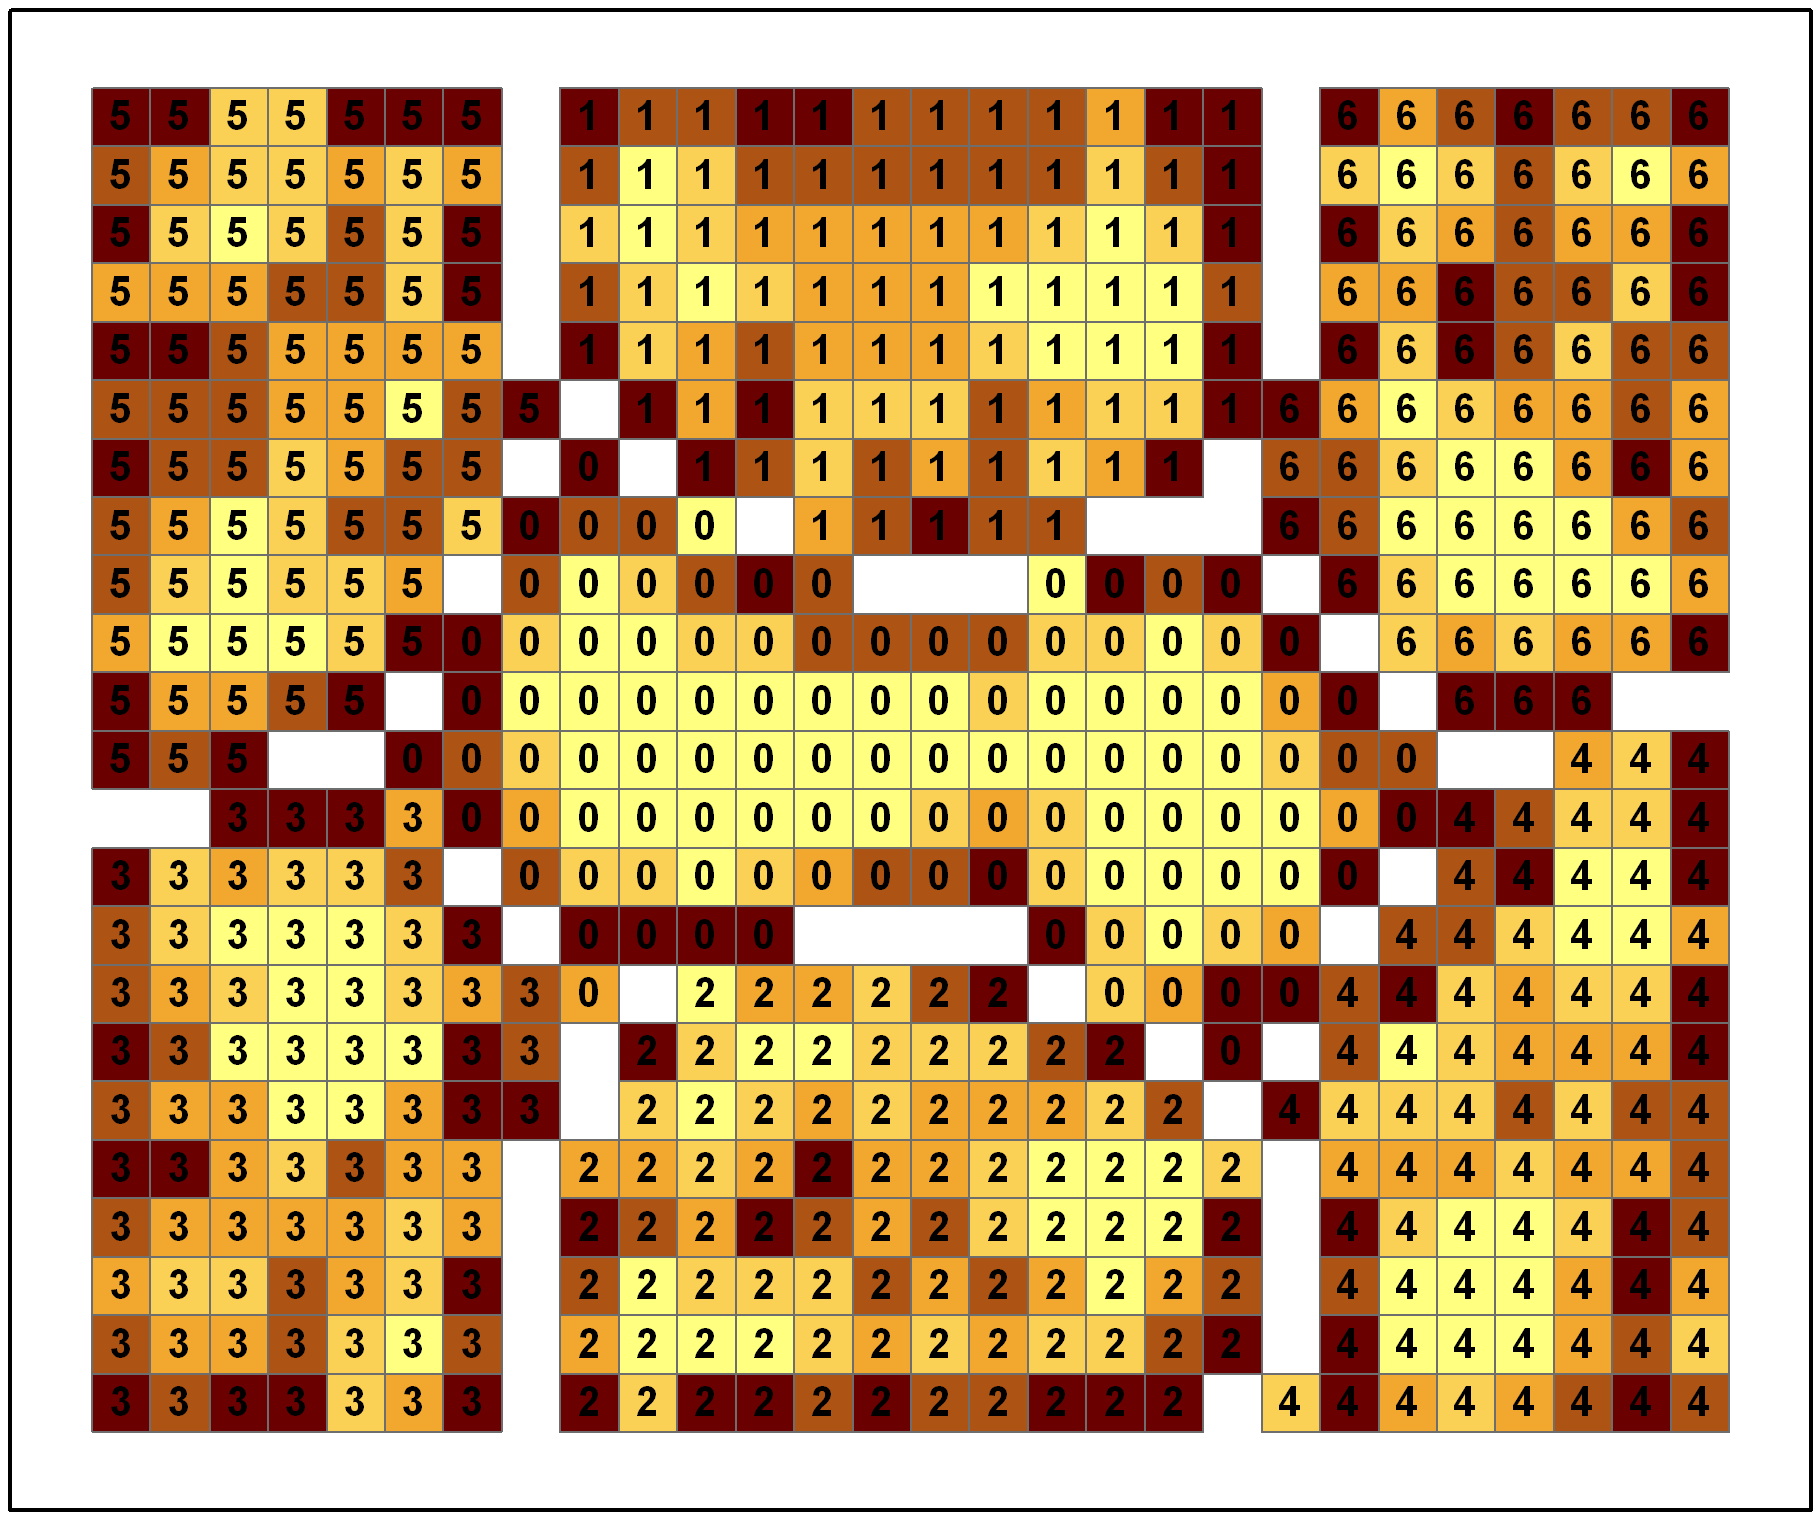
\includegraphics[width=0.7\linewidth]{rook_clusters.png}
%}
\subfigure[Hexagonal Topology]{
  \label{cluster:hex}
  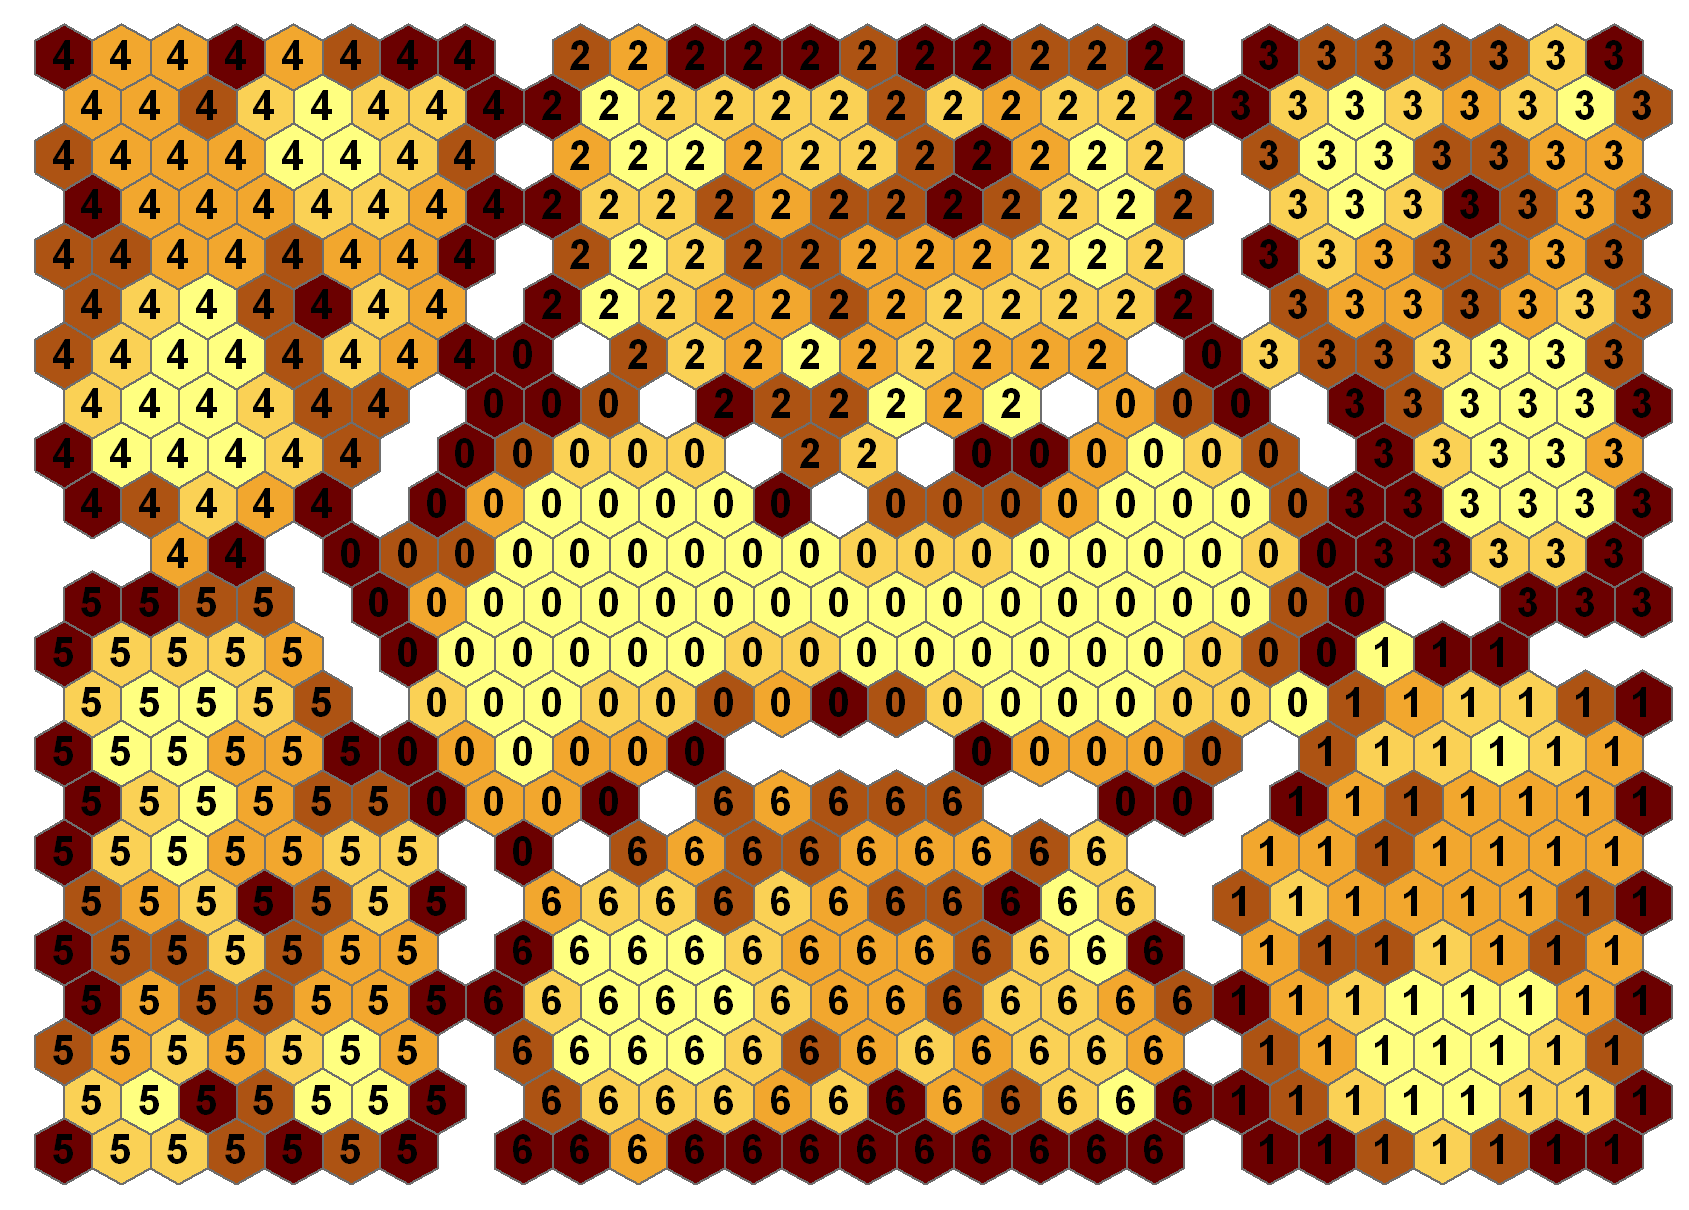
\includegraphics[width=0.85\linewidth]{hex_clusters_no_border.png}
}
%\subfigure[Spherical Topology]{
%  \label{cluster:graph}
%  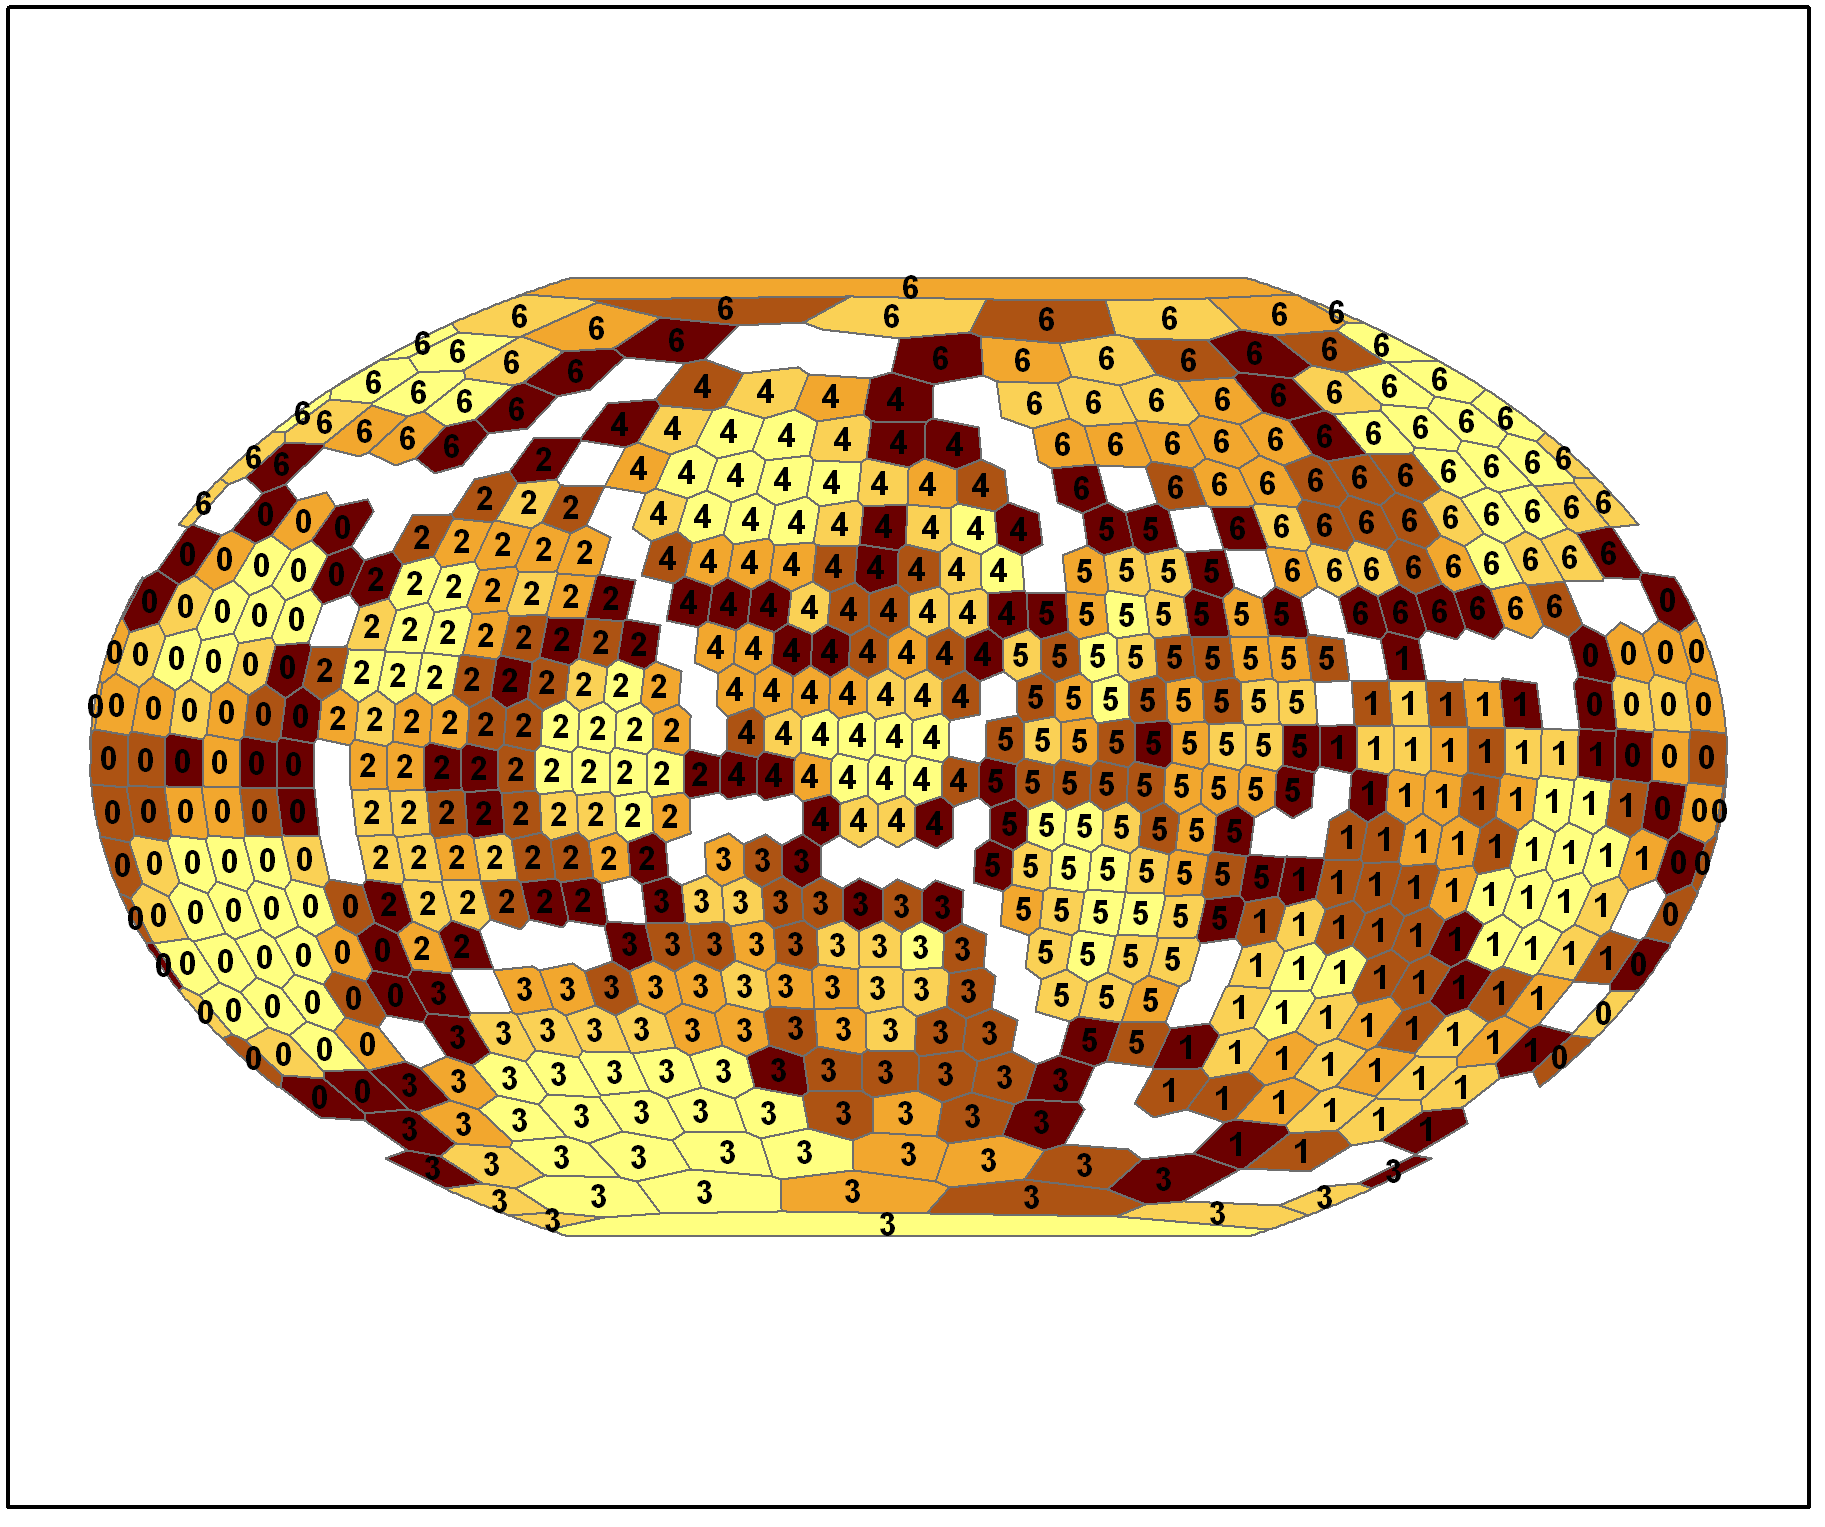
\includegraphics[width=0.7\linewidth]{sphere_clusters.png}
%}
\subfigure[Geodesic Sphere Topology]{
  \label{cluster:geodesic}
  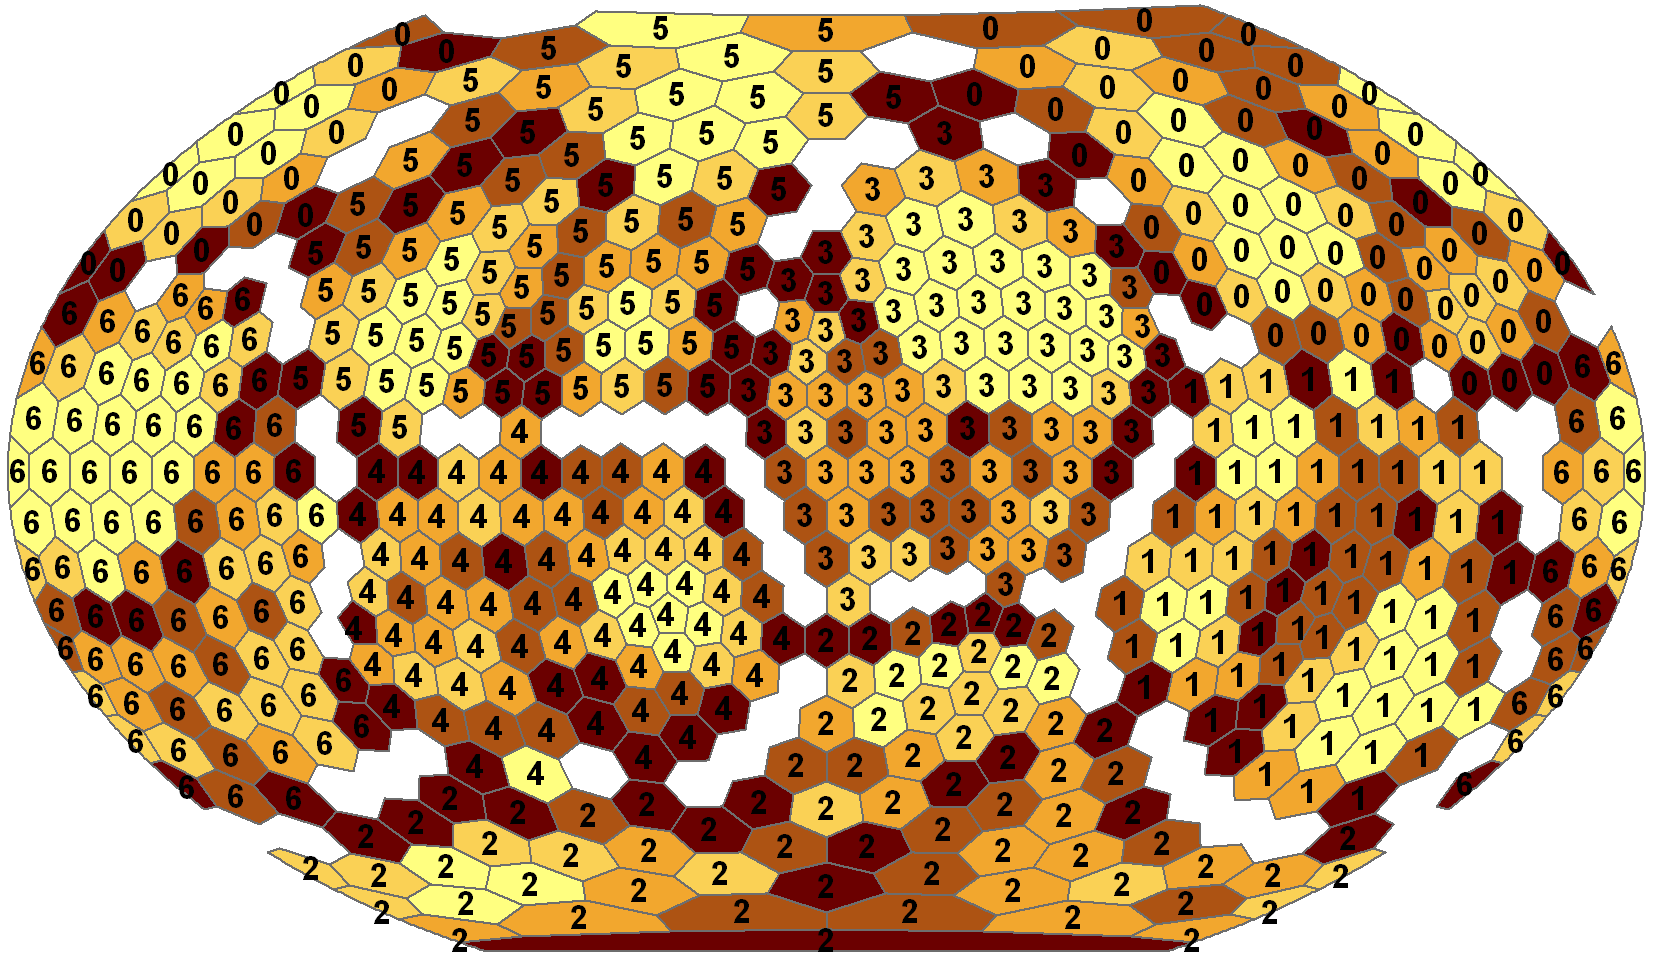
\includegraphics[width=0.85\linewidth]{geodesic_clusters_no_border.png}
}
\label{cluster}
\end{figure}

The internal heterogeneity for the hexagon and geodesic topologies is visualized
in Figure \ref{cluster}.  Neurons are represented as their voronoi regions.
Darker neurons had higher internal heterogeneity.  Each neuron is labled with
the cluster to which the majority of its observation originally belonged. Knowing
which cluster each observation belongs to allows us to see where the clusters
are being mapped to on the trained SOM. It is interesting to note that the
edges of the cluster exhibit higher internal heterogeneity.  This is somewhat
intuitive, as our clusters are normally distributed; the majority of our
observations will fall well within the regions observed in Figure
\ref{cluster}. Each cluster's outliers will be pushed toward the \emph{edges}
of these regions. An observation that is on the edge of a cluster in the
original input-space is further away from the other observations in the
input-space.  Therefore, one would expect that observation to also be near the
edge of a cluster in the SOM space.  In order to represent a three dimensional
cluster in two dimensions, the SOM must compress the edges of the clusters
more than their centers.  This explains the higher internal heterogeneity near
the edges of the clusters.


%\subsection{The Utah-Hawaii Problem}
%\label{states}
 
%In a trained SOM, an earlier observation was made that Utah and Hawaii were similar because they both fell on the same neuron. This raised the question of whether Utah and Hawaii were in fact similar, or if this relationship in the SOM was merely caused by an edge effect.  The answer turns out to be slightly more complicated.  Utah and Hawaii are in fact each other's nearest neighbor, as defined by the census variables used by \cite{skupin08}.  However, as shown in Figure \ref{som:states} and explained in section \ref{bg:edge}, both of these observations can be considered outliers.  Neither fits the trained SOM well and both are far from the mean of all the states.

%In Figure \ref{sphere:states} we present the same data trained on a 400 neuron spherical SOM.  The topology for this SOM is based on \cite{Rakhmanov94}.  We find, not surprisingly, that Utah and Hawaii are separated in this SOM.  This implies that edge effects indeed played a large role in the placement of these two observations in the hexagonal SOM.  As suggested in section \ref{bg:sphere}, we also find these and other outlying observations occupy more space in the trained spherical SOM than in the hexagonal SOM.  States closer to the mean such as Ohio, Missouri and Kentucky are distinctly more clustered in the spherical SOM than in the hexagonal SOM.  It is interesting to note that the orientation between these three states remained largely unchanged between the two maps.
